\documentclass[spanish, 12pt,a4paper]{article}
%\usepackage[spanish]{babel}
\usepackage{algorithmic}
%\usepackage{savesym}
%\savesymbol{IF, algorithmic}
\usepackage[utf8]{inputenc}
\usepackage[spanish]{babel}
\usepackage{aed2-symb}
\usepackage{textcomp}
\usepackage[section, ruled]{algorithm}
\usepackage{hyperref}
\usepackage[pdftex]{graphicx}
\usepackage{epsfig}

\floatname{algorithm}{Algoritmo} % para que diga ``Algoritmo'' y no ``Algorithm''

\renewcommand{\algorithmiccomment}[1]{\ \ \ \textbf{//#1}} %para agregar comntarios en los algoritmos poner
% \COMMENT{ALAN ES GAY}
% \usepackage{algpseudocode}
% \usepackage{lineno}
\newenvironment{parr}
{\begin{list}{}%
         {\setlength{\leftmargin}{2em}}%
         \item[]%
}
{\end{list}}
\newcommand{\tab}{\hspace*{2em}}

\newcommand{\oper}[3]{\samepage\textsc{#1}(#2) $\rightarrow$ \textit{res} $\colon$ #3\\*}
\newcommand{\operL}[3]{\samepage\textsc{#1}(#2) $\rightarrow$ \textit{res} $\colon$ #3}
\newcommand{\operM}[2]{\samepage\textsc{#1}(#2)\\} %�sta es la operaci�n que no devuelve nada
\newcommand{\operMA}[2]{\samepage\textsc{#1}(#2)} %�sta es la operaci�n que no devuelve nada y para usar en el
%``caption'' del ``algorithm''
\newcommand{\vin}[2]{\textbf{in} \textit{#1}$\colon$#2}
\newcommand{\vinout}[2]{\textbf{in/out} \textit{#1}$\colon$#2}
\newcommand{\pre}[1]{\textbf{Pre} $\equiv$ \{#1\}\\*}
\newcommand{\post}[1]{\textbf{Post} $\equiv$ \{#1\}\\*}
\newcommand{\complej}[1]{\textbf{Complejidad:} #1\\*}
\newcommand{\desc}[1]{\textbf{Descripci\'on:} #1\\}
\newcommand{\alias}[1]{\textbf{Aliasing:} #1\\}

% \oper{nombre}{recibe}{devuelve}
% \vin{var}{tipo}
% \vinout{var}{tipo}
% \pre{}
% \post{}
% \complej{O()}
% \desc{txt}
% \alias{txt}

\newcommand{\eqobs}{$=_{obs}$}
\newcommand{\bigo}[1]{O$\big($#1$\big)$}
\newcommand{\NULL}{\textsc{Null} }
\newcommand{\aux}[3]{\samepage #1$\colon$ #2 $\rightarrow$ #3\\*}

\usepackage{hyperref}
\usepackage{color}
\usepackage{graphicx}
\usepackage{graphics}
\usepackage{clrscode3e}
\usepackage{amsthm}
\usepackage{caption}
\usepackage{subcaption}
\usepackage{caratula}
\usepackage{fancyhdr,lastpage}
\usepackage[paper=a4paper, left=1.4cm, right=1.4cm, bottom=1.4cm, top=1.4cm]{geometry}
\usepackage[table]{xcolor} % color en las matrices
\usepackage[font=small,labelfont=bf]{caption} % caption de las figuras en letra mas chica que el texto
				
\color{black}

%%%PAGE LAYOUT%%%
\topmargin = -0.5cm
\voffset = 0cm
\hoffset = 0em
\textwidth = 37em
\textheight = 130 ex
\oddsidemargin = 4 em
\parindent = 2 em
\parskip = 3 pt
\footskip = 7ex
\headheight = 20pt
\pagestyle{fancy}
\lhead{AyED	 III - 2013 C1 - Trabajo Pr\'actico 3} % cambia la parte izquierda del encabezado
\renewcommand{\sectionmark}[1]{\markboth{#1}{}} % cambia la parte derecha del encabezado
\rfoot{\thepage}
\cfoot{}
\numberwithin{equation}{section} %sets equation numbers <chapter>.<section>.<subsection>.<index>

%Lo siguiente controla el ancho de las figuras (principalmente para el texto de los captions)
%\newcommand{\figurewidth}{.9\textwidth}
\newcommand{\figurewidth}{1\textwidth}

\newcommand{\tuple}[1]{\ensuremath{\left \langle #1 \right \rangle }}
\newcommand{\Ode}[1]{\small{$\mathcal{O}(#1)$}}
\newtheorem{teorema}{Teorema}[section]


%El siguiente paquete permite escribir la caratula facilmente
\hypersetup{
  pdftitle={ Algoritmos III - TP1 },
  colorlinks,
  citecolor=black,
  filecolor=black,
  linkcolor=black,
  urlcolor=black 
}

\materia{Algoritmos y Estructuras de Datos III}

\titulo{Trabajo Práctico 1}

\subtitulo{Informe y análisis de resultados.}

%\grupo{Grupo 8}
 
\integrante{Benitti, Raul}{592/08}{raulbenitti@gmail.com}
\integrante{Mengarda,Lucas }{}{l.j.mengarda@gmail.com}
\integrante{Scarpino, Gino}{392/08}{gino.scarpino@gmail.com}
\integrante{Vallejo, Nicolás}{}{nico\_pr08@hotmail.com}
 
\begin{document}
{ \oddsidemargin = 1em
	\headheight = -20pt
	\maketitle
}
	\tableofcontents
	\newpage
	%descripcion de situaciones reales
	\section{Descripción de situaciones reales}

\quad Para ciertos tipos de problemas que se suelen modelar con grafos, se usa coloreo de grafos. Estos problemas, en general, suelen ser donde para ciertas cosas chocan interesas o hay incompatibilidades. Modelandolo, un nodo que representa un objeto está relacionado a otro, es decir, son adyacentes, si pasa lo anteriormente dicho. Coloreando el grafo, los nodos vecinos tienen distinto color, donde el color representa algo oportuno.

\quad

\quad En el caso de este problema, se aplica cuando uno modela un problema con coloreo para el grafo G, cambian las relaciones y se obtiene un grafo H. Se quiere averiguar cómo impacta el cambio, buscando el máximo valor posible. Sirve, de cierta forma, para medir esto.
	\newpage
	%algoritmo exacto
	\section{Algoritmo Exacto}

\subsection{Algoritmo}

\indent La idea de este algoritmo es simple. Recorremos la cantidad de colores posibles del grafo g, calculamos su impacto en h y nos quedamos con el máximo.\\
\indent La dificultad del problema radicaba en calcular la cantidad de colores posibles del grafo, algo que a priori puede ser infinito.\\
\indent Consideramos a los colores como números enteros positivos. De aquí se extrae que hay infinitos colores y por lo tanto infinitos coloreos de G válidos.\\
\indent Sin embargo, se pueden hacer algunas consideraciones para acotar considerablemente la cantidad de colores a usar, sin perder generalidad.\\
\indent En primer lugar, intuitivamente se extrae que con $n$ colores es suficiente, donde $n$ es la cantidad de nodos para analizar todos los casos posibles. Entonces consideraremos como colores los primeros $n$ números enteros positivos. Esto es porque en realidad este caso sirve para analizar aquellos donde se tienen $n$ colores distintos, independientemente de que esos $n$ colores no sean los primeros $n$ números positivos (considerando un color como un número).\\
\indent Sin embargo, todavía se puede acotar un poco más las instancias a analizar.\\
\indent Esto tiene que ver con el hecho de que, aunque definamos $n$ colores, uno podría establecer una biyección entre dos conjuntos de colores con los mismos elementos dónde, por ejemplo, en el conjunto 2 se renombra al color 1 del primer conjunto como el color n y viceversa. Esto provocaría, de no tenerse en cuenta, que se estén analizando casos ya analizados. Si además, en vez de renombrar 2 colores los renombrasemos a todos, estaríamos analizando muchísimos casos que, si bien se corresponden a coloreos distintos, son en el fondo, el mismo caso.\\
\indent Para evitarnos estos análisis de más, determinamos los coloreos de la siguiente manera:\\
\indent Eligimos un nodo cualquiera como el primer nodo para pintar. A ese nodo lo pintamos con el color 1, y por lo que mencionamos anteriormente, de esta manera se estarían analizando también los casos dónde ese nodo tiene otro color entre 2 y n.\\
\indent Ahora se elije otro nodo para pintar en segundo lugar. Para pintarlo tenemos dos posibilidades: o pintarlo del mismo color que el nodo 1 o pintarlo con un color nuevo. Luego, se están generando dos coloreos distintos, y cada uno se sigue generando por separado.\\
\indent La idea es que al pintar el nodo $k$, con $k<=n$, uno podría elegir 2 caminos : o pintarlo de un color ya usado, o pintarlo con un color nuevo.\\
\indent Definamos $max$ como el color de máximo valor utilizado hasta ahora en el coloreo. Luego, existen $max+1$ maneras de continuar ese coloreo, pintando el nodo $k$ de 1,2...$max$ o de un color nuevo, $max+1$.\\
\indent Debe notarse entonces, que por cada paso del coloreo se generan muchos nuevos coloreos más.\\
\indent A medida que se generan los coloreos, generamos otra poda: aquella que determina si al pintar a un nodo de un color se está generando un coloreo válido. En caso de no serlo se deja de analizar ese caso.\\
\indent Luego, de todos los colores posibles válidos se calcula el impacto en H y nos quedamos con aquél que proporciona un máximo impacto.\\

\indent El pseudocódigo del algoritmo es el siguiente:\\   





\begin{algorithm}[H]
\caption{} 
\begin{codebox}
\Procname{$\proc{maximoImpactoExacto}(Grafo$ g$, Grafo$ h$)$}

\li vector$<$unsigned int$>$ $res(n+1)$
\li int $res[0] \gets 0$
\li vector$<$unsigned int$>$ $coloreo(n,0)$
\li $coloreo[0] \gets 1$
\li $colorear(1,g,h,coloreo,res)$
\li	return $res$
\End
\end{codebox}
\end{algorithm}


\begin{algorithm}[H]
\caption{} 
\begin{codebox}
\Procname{$\proc{colorear}(unsigned$ $int$ nodo, $Grafo$ g$, Grafo$ h$, $vector$<$unsigned int$>$ coloreo$, $vector$<$unsigned int$>$ solucion$)$}

\li \If (nodo $>$ n) \Do
\li 	$int$ temp $\gets$ impacto(h, coloreo)
\li		\If $temp > solucion[0]$ \Do
\li			$solucion[0] \gets temp$
\li			\For i desde 0 hasta n \Do
\li				$solucion[i+1]=coloreo[i]$
			\End
		\End
	\End
\li \Else \Do
\li		$int$ maxColor $\gets $ maximo color usado hasta el momento 	
\li		\For c desde 1 hasta maxColor \Do
\li			\If es legal pintar el nodo $nodo$ del color c \Do
\li				vector$<$unsigned int$>$ nuevoColoreo(coloreo)
\li             $nuevoColoreo[nodo] \gets c$
\li             $colorear(nodo+1,g,h,nuevoColoreo,solucion)$
             \End
         \End
\End
\end{codebox}
\end{algorithm}


\subsection{Análisis de complejidad}

\indent Al momento de hacer este análisis de complejidad se tuvieron en cuenta algunas consideraciones.\\
\indent En primer lugar, llamaremos $m$ al máximo entre la cantidad de aristas del grafo G y del grafo H  y $n$ a la cantidad de nodos de dichos grafos.\\
\indent En segundo lugar, en el análisis de complejidad de la función $colorear$ se definirá $k$ como la cantidad de nodos que quedan por pintar hasta ese paso de la recursión, en contraste con la implementación donde la recursión es , por así decirlo $hacia arriba$, significando esto que se inicia desde el primer nodo y se va hacia el último.\\

\indent Analicemos primero la función $colorear$. Como mencionamos anteriormente, consideraremos la recursión en la cantidad de nodos que quedan por colorear.

\indent El caso base será cuando no hayan más nodos por pintar. En dicho caso, el algoritmo simplemente calcula el impacto de dicho coloreo en el grafo H y en caso de ser el de máximo impacto hasta el momento se reemplaza la solución anterior por la nueva. Esto cuesta O(n+m), que es lo que cuesta calcular el impacto en H.\\
\indent Para el caso en el que la cantidad de nodos a pintar sea distinta de cero, el algoritmo calcula los posibles colores con los que pintar el nodo. Esto lo hace buscando cuál es el máximo color usado hasta el momento. El nuevo nodo podrá ser pintado de los colores usados anteriormente o del máximo color usado hasta el momento + 1, es decir pintándolo de un nuevo color. Esto se calcula en tiempo O(n).Luego se llamará a la función recursivamente una cantidad de veces igual al máximo color a utilizar. Ese valor se puede acotar para todos los casos por n-k+1.\\
\indent Además se chequea que agregar ese color genere un coloreo válido, y eso cuesta O(cantidad de vecinos del nodo), que lo podemos acotar por la cantidad de aristas de G, es decir O(m). Luego se hace la llamada recursiva para la instancia inmeditamente menor.\\
\indent Pasando en limpio, en el paso $k$ el algoritmo cuesta (n-k+1)*(n+m + T(k-1)).\\
\indent Es decir:\\

\indent T(0)=n+m\\
\indent T(k)=(n-k+1)*[(n+m)+ T(k-1)]\\

donde $k$ es la cantidad de nodos que quedan por pintar.\\


\indent Veamos entonces cuánto cuesta pintar todos los nodos.\\
\indent Basado en la definición que dimos antes, si tenemos que pintar todos los nodos, estamos en el caso T(n).\\

\indent T(n)=(n-n+1)*(n+m + T(n-1))\\

\indent Desarrollemos T(n):\\


\begin{centering}
T(n)=(n-n+1)*(n+m + T(n-1))=\\
= n+m + [2*(n+m) + 2*T(n-2)]=\\
=(n+m)+2*(n+m) + 2*[3*(n+m)+ 3* T(n-3)]=\\
=(n+m)+2*(n+m)+ 2*3*(n+m) + 2*3 T(n-3)=\\
=(n+m)+2*(n+m)+ 2*3*(n+m) + 2*3*[4*(n+m)+4*T(n-4)]=\\
=(n+m)+2*(n+m)+2*3*(n+m)+2*3*4*(n+m)+ 2*3*4*T(n-4)=\\
=...=\\
=[ $\sum_{i=1}^{n} i! * (n+m) $] + n! * T(0)= \\
=[ $\sum_{i=1}^{n} i! * (n+m) $] + n! * (n+m)\\
\end{centering}


\indent Es decir que T(n)= [ $\sum_{i=1}^{n} i! * (n+m) $] + n! * (n+m)\\

\indent Conjeturamos entonces que T(n) es O($\sum_{i=1}^{n} i! * (n+m) $).\\

\indent Veámoslo por inducción en la cantidad de nodos por pintar:\\

\indent Queremos ver que existe un $d$ real positivo y $n_{0}$ natural positivo tales que para todo $n\geq n_{0}$ vale que $T(n) \leq d * [\sum_{i=1}^{n} i! * (n+m)] $.

\indent Caso base: n=1 \\

\begin{center}
T(1)= $\sum_{i=1}^{1} i! * (1+m)  1! * (1+m) $ = 2*1!*(1+m) =\\
=2*(1+m) $\leq$ 2*  $\sum_{i=1}^{1} i! * (1+m)$ \\
\end{center}

\indent Es decir que con un $d=2$ nos alcanza.\\


\indent Paso inductivo: Suponiendo que vale que $T(n-1) \leq d * [\sum_{i=1}^{n-1} i! * (n-1+m)] $ quiero ver que vale $T(n) \leq d * [\sum_{i=1}^{n} i! * (n+m)] $ \\


\begin{center}
T(n)=(n-n+1)*(n+m + T(n-1))=\\

= (n+m) + T(n-1)$\leq$\\

$\leq$ por hipótesis inductiva $\leq$\\

$\leq n+m + d * [\sum_{i=1}^{n-1} i! * (n-1+m)] \leq \\$

$\leq n+m + d * [\sum_{i=1}^{n-1} i! * (n+m)] \leq$ \\

$\leq (n+m) *[ (d* \sum_{i=1}^{n-1} i!) + 1] \leq$ \\

$\leq (n+m) *[ (d* \sum_{i=1}^{n-1} i!) + n!] \leq$ \\

$\leq (n+m) *[ (d* \sum_{i=1}^{n} i!)] \leq$\\

$\leq  d* \sum_{i=1}^{n} i!*(n+m)$\\

\end{center}

\indent que es lo que queríamos ver.\\

\indent Luego, colorear cuesta O($\sum_{i=1}^{n} i! * (n+m) $).\\

\indent maximoImpactoExacto cuesta entonces O(n+1 + n + 1 + $\sum_{i=1}^{n} i! * (n+m) $) que es O($\sum_{i=1}^{n} i! * (n+m) $).\\

\subsection{Experimentación y Resultados}

	\newpage
	%goloso
	\section{Heurística Constructiva Golosa}

\subsection{Algoritmo}



\quad Analizando las características del problema implementamos una heurística constructiva golosa con los siguientes objetivos:

\quad

\quad \quad \quad - Empezar con el impacto máximo posible (cantidad de aristas de H)

\quad 

\quad \quad \quad - Modificar la menor cantidad de nodos posibles

\quad

\quad \quad \quad - El nodo que se modifique, tendría que bajar lo menos posible el impacto

\quad

\quad Pseudocódigo:

\begin{algorithm}[H]
\caption{} 
\begin{codebox}
\Procname{$\proc{maximoImpactoGoloso}(Grafo$ g$, Grafo$ h$, double porcentaje)$}

\li vector$<$unsigned int$>$ $res(n+1)$
\li int $solucion[0] \gets 0$
\li vector$<$unsigned int$>$ $coloreo(n,1)$
\li vector$<$bool$>$ $modificados(n,false)$
\li \While not G.coloreoLegal(coloreo)) \Do
\li nodo $ \gets $ siguienteModificable(G,H,modificados,porcentaje)
\li \For c desde 1 hasta colores.size() \Do
\li \If G.colorLegalDelNodo(nodo,coloreo,c)
\li coloreo$ [nodo] \gets $ c
\li exitFor
\End
\End
\End
\li $solucion[0] \gets$ impacto(h, coloreo)
\li \For i desde 0 hasta n \Do
		\li $solucion[i+1]=coloreo[i]$
	\End
\li	return $solucion$
\End
\end{codebox}
\end{algorithm}


\begin{algorithm}[H]
\caption{} 
\begin{codebox}
\Procname{$\proc{siguienteModificable}(Grafo$ g$, Grafo$ h,vector$<$bool$>$ modificados, double porcentaje)}

\li vector$<$pair$<$ unsigned int, unsigned int $>$ $>$ posibles
\li \For n nodo in V(G) \Do
\li \If not modificados$ [ $ nodo $ ] $
\li    agregar(posibles,$<$G.impactoNodo(nodo,H,coloreo),nodo$>$)
\End
\End
\li
\li sort(posibles)
\li
\li unsigned int res $ \gets $ random($ \vert $ posibles  $ \vert $ * porcentaje)
\li
\li return res
\End
\end{codebox}
\end{algorithm}

\quad

\quad En \textit{maximoImpactoGoloso} primero se colorea a todos los nodos con el mismo color, por lo que, sin tener en cuenta al grafo G, el impacto en H es máximo. Mientras que no sea legal este coloreo en G, se va a ir modificando los nodos. Apenas se consiga un coloreo legar se detiene. Por lo tanto, no necesariamente el ciclo principal itera la cantidad de nodos (en el peor caso sí).

\quad En \textit{siguienteModificable} se obtiene el nodo a modificar. Se crea una lista de nodos que no hayan sido modificados y se calcula para cada uno su aporte al impacto en H. Se ordena la lista por los siguientes criterios:

\quad

\quad \quad - Menor impacto en H aportado: se desea modificar al que menos aporta para ver si cambiando de color aporta más.

\quad

\quad \quad - Mayor grado en G: se busca que cuanto antes el coloreo de G sea legal modificando lo menos posible, y modificando un nodo de grado grande se podria conseguir esto.

\quad 

\quad \quad - Menor grado en H: por lo que dijimos, en caso de empate de los anteriores criterios, queremos modificar lo menos posible en G y H


\subsection{Análisis de complejidad}

\indent Comencemos analizando la complejidad de la función impactoNodo.\\
\indent Esta función mira para un nodo el impacto que aporta en H, comparando su color con el de sus vecinos. Dicho nodo tiene en H a lo sumo n-1 vecinos. Luego, impactoNodo cuesta O(n).

\indent Analicemos ahora siguienteModificable. Al inicio comienza iterando sobre la cantidad de nodos de H y si dicho nodo no fue modificado o si no tiene vecinos, se calcula el impacto de cada nodo y se lo agrega a un vector de nodos candidatos a ser modificados.En el peor caso, todos los nodos están sin modificar y tienen vecinos,por lo tanto esto cuesta O($n^{2}$).\\
\indent Luego, se ordena de manera creciente el vector de candidatos de acuerdo al impacto de cada nodo.En el peor caso dicho vector tiene n elementos, pues todos los nodos son modificables y ordenarlos cuesta entonces O(n*log(n)).\\
\indent Luego, se itera sobre la cantidad de elementos de ese vector, esta vez para desempatar los nodos. En el peor caso todos los nodos empatan en el impacto que generan. Desempatarlos a todos cuesta en el peor caso O($n^{2}$) , que el caso en el que se invirtió el orden del vector por desempates.\\
\indent A continuación se elige pseudoaleatoriamente en O(1) uno de los primeros elementos del vector.\\
\indent Pasando en limpio, siguienteModificable cuesta O($n^2$ + n*log(n)+ $n^2$), que es O($n^{2}$).\\

\indent Ahora analicemos maximoImpactoGoloso.\\
\indent Al principio realiza unas cuantas operaciones en O(n). De estas es destacable la creación de un vector de tamaño igual al grado del nodo con grado máximo de G, que refiere a la cantidad de colores a usar. Pero el grado máximo de cada nodo es a lo sumo n-1. Luego crear ese vector cuesta O(n).\\
\indent Luego, se ejecuta un while que a lo sumo itera n veces. Esto es porque en el peor caso tuve que pintar todos los nodos de distinto color hasta obtener un coloreo válido.\\
\indent Dentro de ese while está implícito el chequeo de si el coloreo es válido, que cuesta O(n+m), donde vamos a acotar a m como el máximo entre las aristas de G y de H. Se ejecuta siguienteModificable y se itera luego en la cantidad de colores, costando cada iteración en la cantidad de colores O(n) que es lo que cuesta ver si pintar un nodo de ese color es no coincide con el color de uno de los vecinos de ese nodo, que como mencionamos antes pueden ser n-1.\\
\indent Luego, lo de adentro del while cuesta O(n+m+ $n^{2}$) y el costo total del while es de O(n(n+m +$n^{2}$)), que es O(n*(n+m)+ $n^{3}$).\\
\indent Luego de iterar se calcula el impacto de dicho coloreo en O(n+m).\\
\indent Es decir que en total maximoImpactoGoloso cuesta O(n+n*(n+m)+ $n^{3}$ + n+m).\\
\indent Por lo tanto, maximoImpactoGoloso cuesta O(n*(n+m)+ $n^{3}$).\\
 
\subsection{Experimentación y Resultados}
\quad Trabajamos con los siguientes 3 casos: grafos al azar, grafos densos, G y H complementos.

\quad Se midieron los tiempos en corridas de  5 a 100 nodos con 100 repeticiones para cada cantidad de nodos.

\subsubsection{Grafos al azar}

\begin{figure}[H]
	\centering
	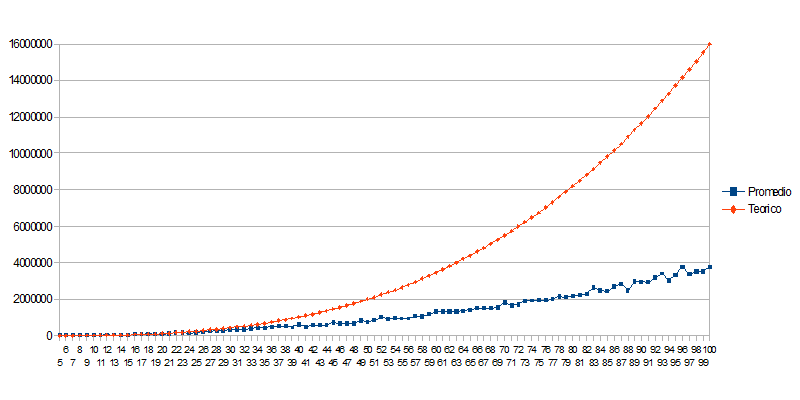
\includegraphics[scale=0.5]{goloso tiempos Azar.png}
\caption{Costos}
\end{figure}

\subsubsection{Grafos densos}

\begin{figure}[H]
	\centering
	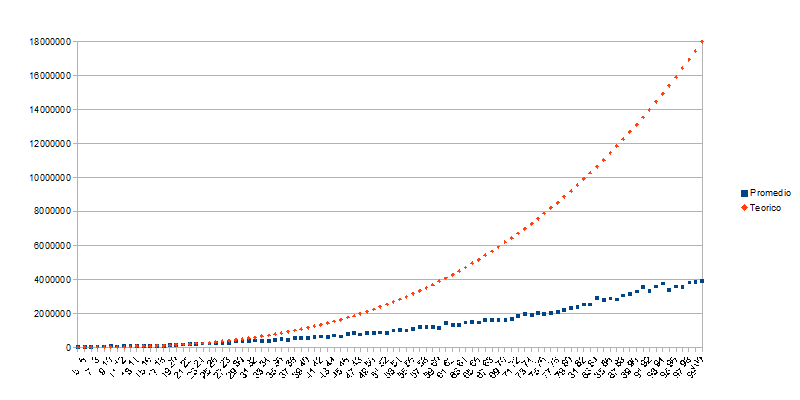
\includegraphics[scale=0.5]{goloso tiempos G y H densos.png}
\caption{Costos}
\end{figure}

\subsubsection{G y H complementos}

\begin{figure}[H]
	\centering
	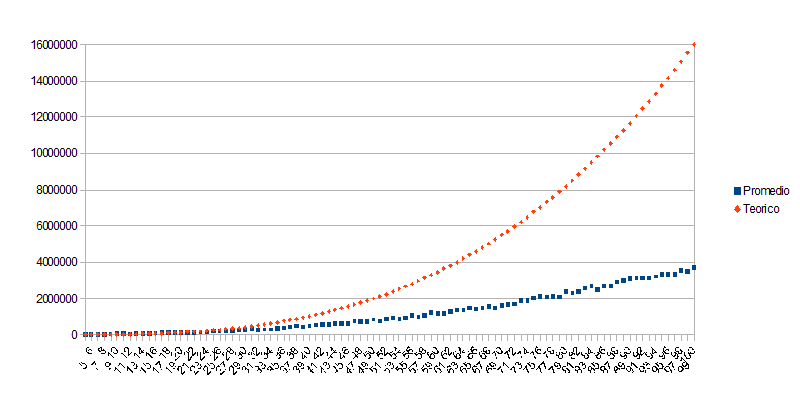
\includegraphics[scale=0.5]{goloso tiempos H complemento.png}
\caption{Costos}
\end{figure}
	\newpage
	%busqueda local
	\section{Heurística de Búsqueda Local}

\subsection{Algoritmo}

\subsection{Análisis de complejidad}

\subsection{Experimentación y Resultados}

	\newpage	
	%grasp
	\section{Metaheurística de Grasp}

\subsection{Algoritmo}

\indent Nuestra implementación de Grasp opera de la siguiente manera: Se generan una cantidad de veces determinada por parámetro de soluciones con nuestra implementación de la heurística golosa. Luego se elige una de ellas pseudoaleatoriamente y se le aplica nuestra implementación de búsqueda local. Si esa solución obtenida con búsqueda locar mejora la que teníamos anteriormente, nos quedamos con ella. Este proceso se iterará una cantidad de veces máxima determinada por parámetro. Sin embargo, puede ocurrir que se deje de iterar antes, si no se encontraron mejores en una cantidad determinada de iteración, también provista por parámetro. A continuación detallamos más detenidamente nuestra implementación.\\

\indent El comportamiento de nuestra implementación de Grasp se ve fuertemente influenciado por ciertos parámetros. A saber, estos son: $porcentaje$, que se usará para obtener las soluciones con nuestras implementaciones del algoritmo goloso y de búsqueda local; $maxRCL$, que determinará la cantidad de candidatos obtenidos mediante la aplicación del algoritmo goloso; $maxIteraciones$ que determinará la cantidad de veces máxima que iterará el algoritmo en el peor caso; y finalmente $maxIterSinMejora$ que determinará la máxima cantidad de iteraciones que permitiremos ejecutarse sin que se obtenga una mejor solución antes de dejar de iterar (donde una mejor solución es aquella que mejora el impacto del coloreo de G en H). \\
\indent Como se puede observar, los últimos dos parámetros descriptos se utilizarán como criterios de parada: a lo sumo el algoritmo iterará $maxIteraciones$ de veces en busca de soluciones, a menos que en una cantidad de iteraciones consecutivas igual a $maxIteracionesSinMejora$ no se obtenga una solución que implique un mayor impacto del coloreo de G con esa solución en H.\\

\indent El algoritmo iterará, en el peor caso, hasta la máxima cantidad de iteraciones permitidas. En cada iteración, se calculan $maxRCL$ (RCL proviene de Restrictive Candidate List) soluciones con el algoritmo goloso que implementamos, cada una de ellas usando el valor de $porcentaje$, es decir que se calculan $maxRCL$ candidatos golosos a los cuales se les puede aplicar el algoritmo de búsqueda local que diseñamos. De esos candidatos se elige uno pseudoaleatoriamente (en nuestro caso, al implementarlo en C++, hicimos uso de la función rand()). A ese candidato elegido, se le aplica nuestra implementación de búsqueda local, obteniendo así una nueva solución. Si esta solución mejora el impacto de G en H en comparación con la solución que se manejaba hasta el momento, se reemplaza a esa solución vieja por esta nueva y se resetea un contador que contiene la cantidad de veces que se iteró sin lograr una mejora. Caso contrario se aumenta dicho contador y se chequea que no se haya alcanzado la máxima cantidad de iteraciones sin mejoras permitidas, en cuyo caso se dejará de iterar y se devolverá la mejor solución que se obtuvo hasta el momento.\\
\indent Este procedimiento se ejecutará hasta que se cumpla con algunos de los criterios de parada. Cuando uno de ellos se cumpla se devuelve la mejor solución que se obtuvo hasta el momento. Es de notar que en cada iteración se generan $maxRCL$ candidatos golosos nuevos de los cuáles se elige uno para continuar con la búsqueda local.\\
\indent La aleatorización de los candidatos golosos se obtiene mediante una combinación de los parámetros $porcentaje$ y $maxRCL$. El primer parámetro impacta en la solución que devuelve el algoritmo goloso que implementamos como describimos en la sección correspondiente. El segundo parámetro determina la cantidad de soluciones candidatas que se calcularán en un principio. Luego, además, de esos $maxRCL$ candidatos se elegirá uno pseudoaleatoriamente (como mencionamos antes, en nuestra implementación usamos la función rand() de C++).\\

\begin{algorithm}[H]
\caption{} 
\begin{codebox}
\Procname{$\proc{maximoImpactoGrasp}(Grafo$ g$, Grafo$ h$, double $ porcentaje$, unsigned$ $int$ maxIteraciones$, unsigned$ $int$ maxIterSinMejora,$ unsigned$ $int$ maxRCL$)$}

\li vector$<$unsigned int$>$ res(n + 1)
\li res[0] $\gets$ 0
\li unsigned int sinMejora $\gets$ 0
\li
\li vector$<$unsigned int$>$ coloreo(n,1) // Todos los elementos valen 1
\li
\li \For i desde 0 hasta maxIteraciones \Do 
\li vector$<$vector$<$unsigned int$>>$ rcl(maxRCL)
\li 	\For k desde 0 hasta maxRCL \Do
\li 		rcl[k] $\gets$ $maximoImpactoGoloso(g,h, porcentaje)$
		\End
\li
\li		unsigned int e $\gets$ índice de uno de los elementos de rcl elegido al azar
\li
\li 	vector$<$unsigned int$>$ solBusqLocal $\gets$ maximoImpactoLocal(g,h,porcentaje,rcl[e])
\li
\li 	\If solBusqLocal[0]$>$res[0] \Do
\li			res[0] =solBusqLocal[0]
\li
\li			\For k desde 1 hasta n \Do
\li				res[k]=solBusqLocal[k]
\li
			\End
\li			sinMejora$\gets$ 0
		%\End
\li		\Else \Do
\li			sinMejora++;
\li         \If sinMejora == maxIterSinMejora \Do
            
\li                salir del ciclo
            
            \End
        \End

	\End	
\li
\li return res
\End
\end{codebox}
\end{algorithm}

\subsection{Análisis de complejidad}

\indent Analicemos la complejidad de maximoImpactoGrasp. Los primeros pasos del algoritmos son crear unos vectores igual a la cantidad de nodos de los grafos. Eso cuesta O(n) para cada creación de vector.\\
\indent Luego se itera maxIteraciones veces. El costo de cada iteración es el siguiente:\\
\indent Primero se calcular maxRCL veces soluciones con maximoImpactoGoloso, donde maxRCL la cantidad de restrictive candidates list, es decir la cantidad máxima de candidatos golosos a utilizar.Ese ciclo cuesta entonces O(maxRCL*(n*(n+m)+ $n^{3}$) de acuerdo a nuestro análisis de complejidad de maximoImpactoGoloso.\\
\indent A continuación, se elige pseudoaleatoriamente uno de esos candidatos.\\
\indent Una vez elegido un candidato, se aplica maximoImpactoLocal con dicha solución golosa.\\ Por lo que analizamos en la sección correspondiente, esto cuesta O(n*(n+m)+ $n^{3}$ +$ n^{2}$*(n+m)).\\
\indent Una vez hecho esto, se decide si se va a quedar con la nueva solución obtenida con maximoImpactoLocal y esto cuesta O(n).\\
\indent Luego, el ciclo cuesta :\\

O(maxIteraciones* [(maxRCL*(n*(n+m)+ $n^{3})$)+ (n*(n+m)+ $n^{3}$ +$ n^{2}$*(n+m))] )\\

 que además es la complejidad de maximoImpactoGrasp.\\


\subsection{Experimentación y Resultados}



\subsubsection{Optimización de parámetros}

\quad Primero buscamos optimizar los parámetros que utiliza nuestra implementación. Los cuales son el parámetro de la heurística golosa aleatoria que usa como base para ir armando las lista de candidatos, y los criterios de parada de una cantidad máxima de iteraciones y una cantidad máxima de iteraciones sin mejora en la solución que se va obteniendo.

\quad Para testear, medir y generar resultados usamos el concepto de distancia en este caso como la diferencia entre el valor máximo que se obtiene del valor de impacto para determinado grafo y el valor obtenido con la heuristica con ciertos valores de parámetros determinados.

\begin{itemize}

\item \textbf{Parámetro de la Heurística Constructiva Golosoa Aleatoria}

\quad

\quad Usamos como base la herística golosa aleatoria que desarrollamos anteriormente. Variamos el parámetro que recibe desde 0.05 hasta 1 con saltos de 0.05. Recordemos que cuando más chico es el valor, la heuristica golosa elige aleatoriamente entre menos candidatos posibles para ir coloreando, siendo si es valor 1, elige entre cualquier nodo posible.

\quad Testeamos con 50, 100 y 150 nodos y 100 repeticiones para cada cantidad de los mismos. Los grafos elegidos para generar resultados son grafos generados al azar porque generar diversos tipos de grafos.

\quad

\quad Los resultados obtenidos con 50 nodos:

\begin{figure}[H]
	\centering
	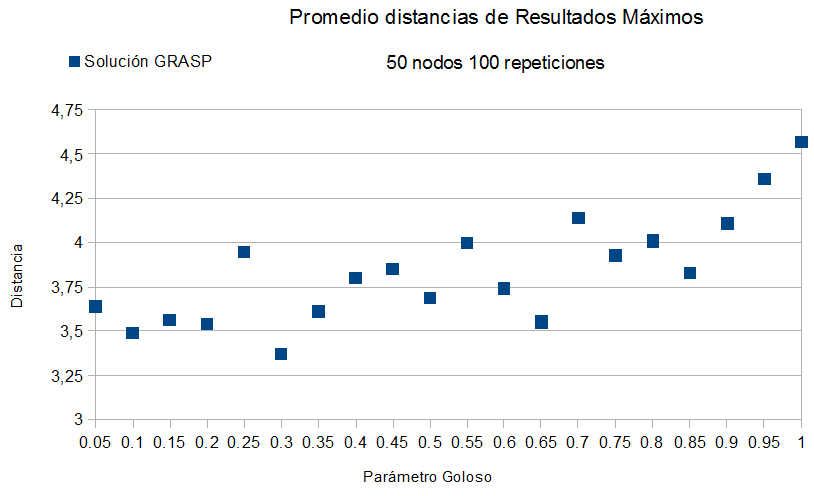
\includegraphics[scale=0.6]{optimizacionGRASPParGoloso1.png}
\end{figure}

\quad

\quad Con 100 nodos no se pudo apreciar diferencias con respecto a lo anterior.

\quad

\quad Los resultados obtenidos con 150 nodos:

\begin{figure}[H]
	\centering
	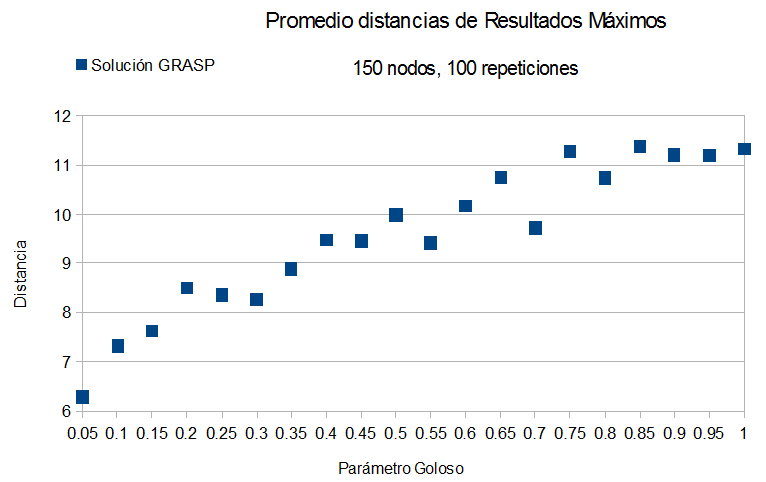
\includegraphics[scale=0.6]{optimizacionGRASPParGoloso2.png}
\end{figure}

\quad Tras obtener estos resultados, decidimos que cuando el grafo posea menos de 50 nodos el valor sea 0.3, en cambio, cuando tenga más nodos sea de 0.1. Esto significa que cuando más \textit{chico} es el grafo, en el goloso aleatorio se elige al azar entre menor cantidad de nodos para colorear de cierta forma. Osea que cuando se construye nuestra lista de candidatos posibles, cuanto más \textit{grande} es el grafo, se necesita menor porcentaje de aleatoriedad para crear posibles soluciones distintas entre si.

\quad

\item \textbf{Parámetro Cantidad Máxima de Iteraciones}

\quad

\quad Como en nuestra implementación, este criterio de parada depende de la cantidad de nodos del grafo, decidimos variar para optimizarlo con los valores de 0.5 hasta 5, con pasos de 0.5. Es decir, es un coeficiente que multiplica la cantidad de nodos: siendo 2 se itera 2 veces la cantidad de nodos, y cuando es 5 se itera 5 veces la cantidad de nodos. Elegimos ese rango porque tenemos en cuanta que cuantas más iteraciones, más es el costo computacional de la heuristica.

\quad Al igual que antes testeamos con 50, 100 y 150 nodos y 100 repeticiones para cada cantidad de los mismos. Los grafos elegidos para generar resultados son grafos generados al azar porque generar diversos tipos de grafos.

\quad Lo que obtuvimos en promedio:

\begin{figure}[H]
	\centering
	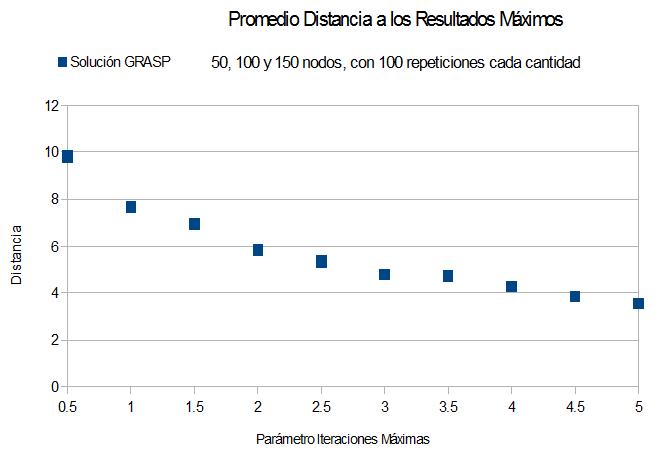
\includegraphics[scale=0.6]{optimizacionGRASPParIterMax.png}
\end{figure}

\quad Se puede observar que a partir del valor 3 del parámetro, lo que se mejora de la soluciones que se van obteniendo es menos. Creemos que es el punto ideal entre costo computacional y mejora de las soluciones parciales. Sin embargo, cuando son grafos pequeños, la cantidad de iteraciones es poca por lo que probamos con menor cantidad de nodos y un rango para el parámetro mayor. Obtuvimos que lo óptimo sería el valor 5.

\begin{figure}[H]
	\centering
	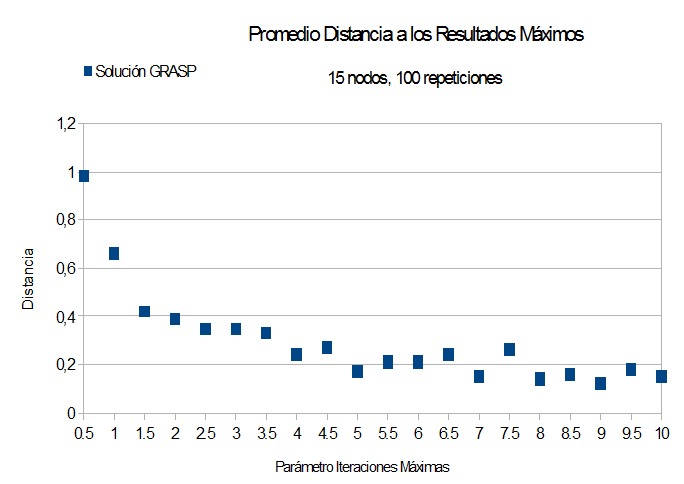
\includegraphics[scale=0.6]{optimizacionGRASPParIterMax2.png}
\end{figure}

\quad Aumentar el valor del parámetro de 3 a 5 no implicaria un gran costo computacional debido a que es menor la cantidad de nodos. Entonces queda que para grafos de menos de 50 nodos se utiliza la herística con cantidad máxima de iteraciones 5 veces la cantidad de nodos. Con grafos \textit{más grandes} se utiliza 3 veces la cantidad de nodos.

\item \textbf{Parámetro Cantidad de Iteraciones Máximas Sin Mejora}

\quad

\quad Con este criterio de parada, determinamos si pasa cierta cantidad de iteraciones sin que se haya mejorado la solucón parcial obtenida, se finaliza. Este parámetro determina el porcentaje de las iteraciones máximas que tienen que pasar sin que se mejore para terminar. Por eso, los rangos posibles que definimos son de 0.1 a 0.9.

\quad Al igual que con los otros dos parámetros, probamos con grafos aleatorios de 50,100 y 150 nodos con 100 repeticiones para cada cantidad.

\begin{figure}[H]
	\centering
	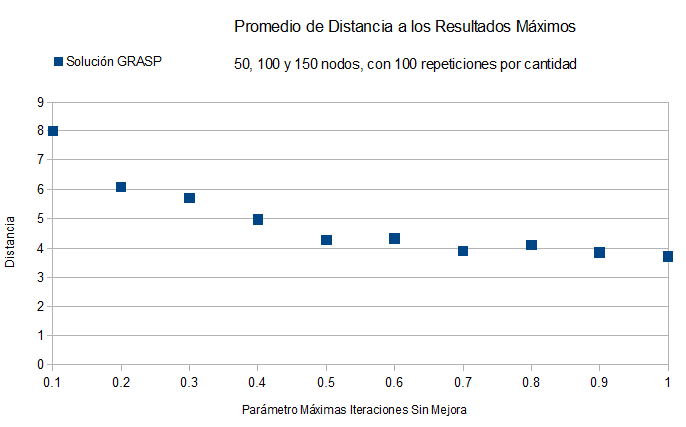
\includegraphics[scale=0.6]{optimizacionGRASPParIterMaxSinMejora.png}
\end{figure}

\quad Podemos observar como a partir del valor 0.5, se estabiliza la mejora por lo que consideramos a ese valor como el óptimo. Es decir, que si no se obtiene una mejora en la solución parcial obtenida en esa cantidad de iteraciones se termina, osea, la mitad de la cantidad máxima de iteraciones de la heurística. Ejemplo: si son 500 iteraciones máximas, si se cumple que en 250 iteraciones consecutivas no hay mejora, se finaliza.

\end{itemize}

\subsubsection{Costo temporal}

\quad Vamos a comparar el costo obtenido por nuestra heuristica versus el costo calculado teóricamente en la sección de complejidad.

\quad Vamos a testear con 3 tipos de grafos: al azar, grafos estrellas no uniformes, grafos redes de 4 vértices.
	\newpage
	%experimentacion
	\section{Experimentación General}

	\newpage
	\bibliographystyle{plain}	
	\clearpage
	\addcontentsline{toc}{section}{Bibliography}
%	\bibliography{bib}	
\end{document}

